%%%%%%%%%% Quotients %%%%%%%%%%
\chapter{ Quotient Groups}
\label{QuotientGrps}
% use \chaptermark{}
% to alter or adjust the chapter heading in the running head
\section{ Cosets}

\begin{definition}[Left Cosets]
        Let $H \leq G$ be a subgroup, $g \in G$. The \Emph{left coset} of $H$ containing $g$, or generated by $g$, is \begin{equation}
                gH := \{g\star h:h\in H\}\subseteq G
        \end{equation}
\end{definition}
\begin{enumerate}
        \item[$\rightarrow$] Notation depends on the operation: $g+H, g\star H, gH, etc.$
\end{enumerate}

\begin{note}
        For $H \leq G$ and all $g \in G$, $g = g\star e_G \in gH$ since $e_G \in H$. If $g \in H$, $gH = H$, as $h = g \star (g^{-1} \star h)$ for all $h \in H$. Hence we can have $gH = g'H$ for $g \neq g'$. Note $gH$ is only a subgroup if $g \in H$ so $gH = H$.
\end{note}

\begin{example}
        Take $G = \Z/4\Z$, $H = \langle [2]\rangle \leq G$. So $H = \{[0], [2]\}$. Then we have the cosets \begin{table}[H]
                \centering
                \begin{tabular}{cc}
                        $g$ & $gH = g+H$ \\
                        $[0]$ & $H$ \\
                        $[1]$ & $\{ [1],[3] \} = [1] +H$\\
                        $[2]$ & $H$ \\
                        $[3]$ & $\{[3], [1]\} = [3]+H = [1] +H$
                \end{tabular}
        \end{table}
        we have $H = [2]+H$ and $[1]+H = [3]+H$, so we get 2 distinct left cosets and they form a partition of $G$.
\end{example}

\begin{lemma}
        The left cosets of $H \leq G$ form a partition of $G$.
\end{lemma}
\begin{proof}
        First, as $g \in gH$ for all $g \in G$ we have that $$\bigcup\limits_{g\in G}gH = G$$
        Then, suppose $gH\cap g'H \neq \emptyset$, and let $gh = g'h' \in gH\cap g'H$. Then $g = g'h'h^{-1} \in g'H$ and $g' = gh{h'}^{-1} \in gH$. Then, for all $gh'' \in gH$ and $g'\overline{h} \in g'H$, $gh'' = g'(h'h^{-1}h'') \in g'H$ and $g'\overline{h} = g(h{h'}^{-1}\overline{h}) \in gH$, so $g'H \supseteq gH$ and $g'H \subseteq gH$. Thus $g'H = gH$, so by proof by contrapositive we have that all distinct cosets are disjoint, completing the proof.
\end{proof}

\begin{remark}
        The left cosets of $H$ are the equivalence classes for the equivalence relation \begin{equation}
                a \equiv \iff a^{-1}b \in H
        \end{equation}
\end{remark}

\begin{definition}[Index]
        The number of left cosets of $H$ in $G$ is called the \Emph{index} of $H$ in $G$, denoted by \begin{equation}
                |G:H|\;or\;[G:H]
        \end{equation}
\end{definition}


\begin{lemma}
        For all $g \in G$, $G$ a group, and all $H \leq G$, $|gH| = |H|$.
\end{lemma}
\begin{proof}
        Define the map $\phi:H\rightarrow gH$ by $h \mapsto gh$. Then $\phi$ is a bijection with inverse $\varphi:gH\rightarrow H$ defined by $gh \mapsto g^{-1}gh$. Indeed, we have $\varphi \circ \phi(h) = \varphi(gh) = g^{-1}gh = h$. Thus, by definition of cardinality of sets $|H| = |gH|$.
\end{proof}



\begin{definition}
        Let $G$ be a group with $H \leq G$. $g \in G$ is a \Emph{representative} of a left coset $xH$ of $H$ in $G$ if and only if $g \in xH$ ($\iff gH = xH$). A \Emph{complete set of representatives} of the left cosets of $H$ in $G$ is a set $S \subseteq G$ such that $S$ contains one, and only one, representative of each left coset of $H$ in $G$.
\end{definition}

\begin{example}
        \leavevmode
        \begin{enumerate}
                \item For $n \geq 1$, and $H = n\Z \leq \Z =G$, a number $m \in \Z$ is a representative of $a + n\Z$ if and only if $n\;\vert\;m-a$. A complete set of representatives would be $\{0,1,2,...,n-1\}$ of the left cosets of $n\Z$ in $\Z$.
                \item Consider $H = \{g\in\C^{\times}:|g| = 1\}\leq \C^{\times}$.
                        \begin{center}
							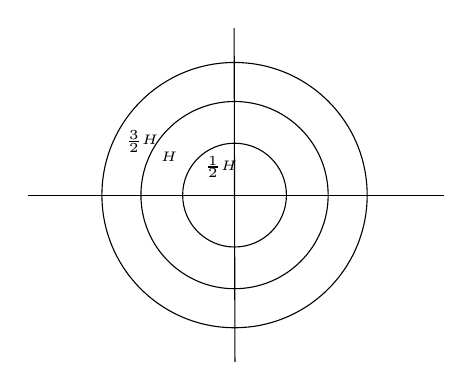
\begin{tikzpicture}[x=0.75pt,y=0.75pt,yscale=-1,xscale=1]
								%uncomment if require: \path (0,310); %set diagram left start at 0, and has height of 310

								%Straight Lines [id:da5661096376446424] 
								\draw    (90,160.2) -- (290.4,160.2) ;
								%Straight Lines [id:da14833488359267633] 
								\draw    (189.2,79.8) -- (189.6,240.6) ;
								%Shape: Circle [id:dp40139760849871564] 
								\draw   (164.4,160.2) .. controls (164.4,146.39) and (175.59,135.2) .. (189.4,135.2) .. controls (203.21,135.2) and (214.4,146.39) .. (214.4,160.2) .. controls (214.4,174.01) and (203.21,185.2) .. (189.4,185.2) .. controls (175.59,185.2) and (164.4,174.01) .. (164.4,160.2) -- cycle ;
								%Shape: Circle [id:dp7821381105807637] 
								\draw   (144.3,160.2) .. controls (144.3,135.29) and (164.49,115.1) .. (189.4,115.1) .. controls (214.31,115.1) and (234.5,135.29) .. (234.5,160.2) .. controls (234.5,185.11) and (214.31,205.3) .. (189.4,205.3) .. controls (164.49,205.3) and (144.3,185.11) .. (144.3,160.2) -- cycle ;
								%Shape: Circle [id:dp9798232031691783] 
								\draw   (125.5,160.2) .. controls (125.5,124.91) and (154.11,96.3) .. (189.4,96.3) .. controls (224.69,96.3) and (253.3,124.91) .. (253.3,160.2) .. controls (253.3,195.49) and (224.69,224.1) .. (189.4,224.1) .. controls (154.11,224.1) and (125.5,195.49) .. (125.5,160.2) -- cycle ;

								% Text Node
								\draw (173.8,140.2) node [anchor=north west][inner sep=0.75pt]  [font=\tiny]  {$\frac{1}{2} H$};
								% Text Node
								\draw (152.6,138.2) node [anchor=north west][inner sep=0.75pt]  [font=\tiny]  {$H$};
								% Text Node
								\draw (135.8,127.8) node [anchor=north west][inner sep=0.75pt]  [font=\tiny]  {$\frac{3}{2} H$};


							\end{tikzpicture}
						\end{center}
				A complete set of representatives is $\R_{>0}$. Indeed, the map \begin{equation}
					\map{\R_{>0}\xrightarrow{f}\{\text{left cosets of $H$ in $\C^{\times}$}\}}{r\mapsto rH}
				\end{equation}
				Indeed, for all $x \in \C^{\times}$ $x = re^{i\theta}$ so $xH = re^{i\theta}H = rH$, as $e^{i\theta} \in H$, so $f$ is surjective. If $r,r' \in rH$ then $r' = rz$ with $|z| = 1$, so $|r'| = |rz| = |r|$. But, for $r,r' \in \R_{>0}$ $|r'| = |r|$ implies $r' = r$. Thus, $f$ is a bijection.
			\item Consider $H = \R\leq \C$. Then $\R$ identified with the y axis is a complete set of representative under the map \begin{equation}
				\map{\R\mapsto\{\text{left cosets of $H$}\}}{r\mapsto ir+R}
			\end{equation}
			\item Consider $\R^{\times} \leq \C^{\times}$. Then $[0,\pi[$ is a complete set of representatives, with the map \begin{equation}
				\map{{[0,\pi[}\rightarrow\{\text{left cosets of $\R^{\times}$}\}}{\theta \mapsto e^{i\theta}\R^{\times}}
			\end{equation}
		\end{enumerate}
\end{example}

\begin{definition}
        For a subgroup $H \leq G$, a \Emph{right coset} of $H$ in $G$ is a subset of $G$ of the form \begin{equation}
                Hg := \{hg:h\in H\}
        \end{equation}
        We say that $Hg$ is the right coset generated by $g$ or containing $g$.
\end{definition}

\begin{theorem}
        The right cosets of $H$ in $G$ form a partition of $G$.
\end{theorem}
\begin{proof}
        (Left to the reader)
\end{proof}


\begin{remark}
        The right cosets of $H$ in $G$ are the equivalence classes of the equivalence relation \begin{equation}
                a\equiv b \iff ba^{-1} \in H
        \end{equation}
\end{remark}

\begin{proposition}
        There is a bijection \begin{equation}
                \map{\{\text{left cosets of $H$ in $G$}\}\rightarrow \{\text{right cosets of $H$ in $G$}\}}{aH \mapsto Ha^{-1}}
        \end{equation}
\end{proposition}
\begin{proof}
        (Left to the reader)
\end{proof}

\begin{corollary}
        The number of right cosets of $H$ in $G$ is also $|G:H|$, the index.
\end{corollary}


\begin{remark}
        When $G$ is abelian, every right coset $Hg$ is a left coset $gH$.
\end{remark}

\begin{example}[Non-example]
        For $H = \langle y \rangle \leq D_3 = \langle x,y\rangle$, the left and right cosets give two different partitions of $D_3$. Indeed, $H = yH$, $xH = xyH$, and $x^2H = x^2yH$ are the left cosets, while $H = yH$, $Hx = Hx^2y$, $Hx^2 = Hxy$ are the right cosets.
\end{example}


\section{ Lagrange's Theorem and Applications}

\begin{theorem}[Lagrange's Theorem]\label{thmname:lagrange}
        If $H$ is a subgroup of a finite group $G$, then $|H|$ divides $|G|$.
\end{theorem}
\begin{proof}
        Let $H\leq G$ for $G$ finite. Then since the cosets of $H$ partition $G$ we have that \begin{equation}
                |G| = \sum\limits_{cosets}|gH| = \sum\limits_{cosets}|H| = |G:H||H|
        \end{equation}
        so by definition $|H|$ divides $|G|$.
\end{proof}


\begin{example}
        \leavevmode
        \begin{enumerate}
                \item Let $g \in G$ (a finite group). Then $o(g)\;\vert\;|G|$ and thus $g^{|G|} = e_G$.
                        \begin{proof}
                                (Left to the reader)
                        \end{proof}
                \item If $|G| = p$ is prime, then $G$ has only the trivial subgroups, $H = \{e_G\}$ and $H = G$, since $|H|\;\vert\;|G|$ implies $|H| \in \{1,p\}$. Actually:
                        \begin{corollary}
                                If $|G| = p$ a prime, then $G \cong \Z/p\Z$.
                        \end{corollary}
                \item If $|G| = p^2$ for a prime $p$ then either $G \cong \Z/p^2\Z$ or $g^p = e$ for all $g \in G$.
                        \begin{proof}
                                (Left to the reader)
                        \end{proof}
        \end{enumerate}
\end{example}


\begin{remark}
        A class $[m] \in \Z/n\Z$ has a multiplicative inverse if and only if $\gcd(m,n) = 1$ (they are \Emph{relatively prime}).
\end{remark}
\begin{proof}
        If $\gcd(m,n) = 1$ then there exist $a,b \in \Z$ such that $am + bn = 1$, so $[a][m] = [1]$ modulo $n$. On the other hand, if $[a][m] = [1]$ for some $m \in \Z$ then there exists $b \in \Z$ such that $1 = am+bn$. Hence, $m\Z + n\Z = \Z$, so $\gcd(m,n) = 1$.
\end{proof}

\begin{definition}
        Fix an integer $n > 1$. Let $(\Z/n\Z)^{\times}$ be the set of these classes with multiplicative inverses from $\Z/n\Z$ with multiplication. Then, it is a group with identity $[1]$.
\end{definition}

\begin{definition}[Euler Totient Function]
        Let $\varphi(n) :=|(\Z/n\Z)^{\times}|$ (the \Emph{Euler totient function}), or equivalently \begin{equation}
                \varphi(n) := |\{m \in \{0,1,...,n-1\}:\gcd(m,n) = 1\}|
        \end{equation}
        This is also known as the \Emph{Euler phi function}.
\end{definition}

\begin{example}
        Take $p$ a prime. Then \begin{enumerate}
                \item $\varphi(p) = p-1$
                \item $\varphi(p^k) = p^k - p^{k-1}$ for all $k \geq 1$
        \end{enumerate}
\end{example}


\begin{theorem}[Euler's Theorem]
        If $a$ and $n \geq 2$ are relatively prime integers, then \begin{equation}
                a^{\varphi(n)} \equiv 1 \mod n
        \end{equation}
\end{theorem}
\begin{proof}
        (Left to the reader)
\end{proof}

\begin{theorem}[Fermat's Theorem]
        If $p$ is a prime then $a^p = a \mod p$ for all $a \in \Z$.
\end{theorem}
\begin{proof}
        (Left to the reader)
\end{proof}

\subsection{ Classification of Groups of Order 2p for p a prime}

\begin{theorem}
        Let $G$ be a group. If $|G| = 2p$, then either $G$ is cyclic $(\cong \Z/2p\Z)$ or $G$ is isomorphic to the dihedral group $D_p$ of order $2p$.
\end{theorem}
\begin{proof}
        This proof extends over this subsection and will be completed after stating a few lemmas
\end{proof}


\begin{lemma}
        If $G$ is a group in which $g^2 = e_G$ for all $g \in G$, then $G$ is abelian.
\end{lemma}
\begin{proof}
        Let $x,y \in G$. Then $(xy)^2 = e$ since $xy \in G$, so $xy = (xy)^{-1} = y^{-1}x^{-1} = yx$. Thus $G$ is abelian as claimed.
\end{proof}


\begin{proof}[Proof of Theorem for p = 2]
        First, suppose $|G| = 2\cdot 2 = 2^2 = p^2$. Then, by application of \ref{thmname:lagrange} we have $G$ is cyclic or $g^p = g^2 = e_G$ for all $g \in G$. If $G$ is cyclic $G \cong \Z/4\Z$ and we're done. If $G$ is not cyclic, $G = \{e_G,g_2,g_3,g_4\}$. Set $x = g_2$ and $y = g_3$. We have $|G| = 2n$, $x^n = e_G = y^2$ and $yx= xy = x^{-1}y$ since $G$ is abelian by the last Lemma. Thus, we have that $G \cong D_2$, the dihedral group of order $4$.
\end{proof}

\begin{proof}[Proof of Theorem for p > 2]
        If $G$ is cyclic we're done, so suppose $G$ is not cyclic. We must show that $G \cong D_p$. By \ref{thmname:lagrange} $o(g) \in \{1,2,p\}$ for all $g \in G$ (since $G$ is assumed to not be cyclic). 

        \begin{claim}
                $G$ has an element of order $p$.
        \end{claim}
        \begin{proof}
                If $g^2 = e_G$ for all $g \in G$ then $G$ is abelian by the Lemma. Take three distinct elements $\{e_G, a, b\}$ in $G$, so $\{e_G,a,b,ab\} \leq G$, which is isomorphic to $D_2$. But $|D_2| = 4$ and $4 \;\cancel{\vert}\;2p$ as $p > 2$ is odd. Thus, this is not possible by \ref{thmname:lagrange}. Hence, there must exist $x \in G$ such that $o(x) = p$.
        \end{proof}
        Set $H = \langle x \rangle$, so $|H| = o(x) = p$.
        
        \begin{claim}
                If $g \in G$ with $g \notin H$, then $o(g) = 2$.
        \end{claim}
        \begin{proof}
                Note $g \neq e_G$ because $e_G \in H$, so $o(g) \neq 1$. We have that $G = H\coprod gH$ because $|G| = 2p = |H| + |gH|$ and $gH \cap H =\emptyset$ since $g \notin H$ by $g \in gH$. Next, note $g^2 \in gH$ if and only if $g \in H$, so $g^2 \notin gH$, whcih implies $g^2 \in H$. If $o(g) = p$ then $g = g^{p+1} = (g^2)^{\frac{p+1}{2}} \in H$ since $p+1$ is even. But $g \notin H$, so this is a contradiction. Hence, we must have tha $o(g) = 2$.
        \end{proof}

        Now, let $y \in G$ such that $y \notin H$, so $o(y) = 2$. Then we have $\langle x,y\rangle \geq H$ and $\langle x, y \rangle \subseteq yH$. But $G = H\coprod gH$, so $\langle x,y \rangle = G$. Thus $|\langle x,y \rangle| = 2p$. Moreover, $o(x) = p$ and $o(y) = 2$. We want $yx = x^{-1}y$. Note $yx \in yH$ by definition of the left coset, so $(yx)^2 = e_G$. Hence, $yx = (yx)^{-1} = x^{-1}y$ as $y = y^{-1}$. Therefore, $G$ satisfies the criterion for the dihedral group of order $2p$, so $G \cong D_p$.
\end{proof}



\section{ The Alternating Group}

\begin{definition}
        Let $n \geq 1$, $A$ be an $n\times n$ matrix, and let $\sigma \in S_n$. Define an action of $S_n$ on $\GL_n(\R)$ by letting $\sigma(A)$ be the $n \times n$ matrix with the $i$-th row being the $\sigma^{-1}(i)$-th row of $A$. That is \begin{equation}
                \sigma(A)_{\sigma(i)j} = A_{ij} \;or\;\sigma(A)_{ij} = A_{\sigma^{-1}(i)j}
        \end{equation}
        so $\sigma$ sends the $i$-th row of $A$ to the $\sigma(i)$-th row.
\end{definition}

\begin{claim}
        The map defined by \begin{equation}
                \map{S_n\xrightarrow{f}\GL_n(\R)}{\sigma \mapsto \sigma(\id_n)}
        \end{equation}
        is a well defined group homomorphism.
\end{claim}
\begin{proof}
        First, let $\sigma, \eta \in S_n$. I claim $\sigma(A) = \sigma(\id_n)A$ for all $A \in \GL_n(\R)$. Indeed, observe that \begin{align*}
                \left(\sigma(\id_n)A\right)_{ik} &= \sum\limits_{j=1}^n\sigma(\id_n)_{ij}A_{jk} \\
                &= \sum\limits_{j=1}^n\id_{\sigma^{-1}(i)j}A_{jk} \\
                &= \sum\limits_{j=1}^n\delta_{\sigma^{-1}(i)j}A_{jk} \\
                &= A_{\sigma^{-1}(i)k} \\
                &= \sigma(A)_{ik}
        \end{align*}
        where $\delta_{ij} = \left\{\begin{array}{ll} 1, & i = j \\ 0, & i \neq j \\ \end{array}\right.$ is the \Emph{kronecker delta}. Hence we have that \begin{equation}
                f(\sigma)f(\eta) = \sigma(\id_n)\eta(\id_n) = \sigma(\eta(\id_n)) = (\sigma \circ \eta)(\id_n) = f(\sigma \circ \eta)
        \end{equation}
        Thus $f$ is multiplicative. Next we want to show $\det(f(\sigma)) \neq 0$, so $f(\sigma) \in \GL_n(\R)$ for all $\sigma \in S_n$. For $\sigma$ a 2-cycle, (i.e. a transposition) we have $\sigma(\id_n) = E$ an elementary matrix for the elementary operation of type I (exchanging two rows), so $\det(\sigma(\id_n)) = 1$ or $-1$. But, every permutation $\sigma \in S_n$ can be written as a product of transpositions, say $\sigma = \beta_1 \circ ...\circ \beta_r$. Hence, multiplicativity says $f(\sigma) = f(\beta_1)...f(\beta_r)$ where $\det(f(\beta_i)) \in \{1,-1\}$ for all $i$, so $\det(f(\sigma)) \in \{1,-1\}$. Hence we have that $f(\sigma) \in \GL_n(\R)$, completing the proof.
\end{proof}


\begin{corollary}
        Due to this result we have a homomorphism
        \begin{center}
            \begin{tikzpicture}[baseline = (a).base]
            \node[scale = 1] (a) at (0,0){
                \begin{tikzcd}
                        S_n \ar[dr, "f", swap] \ar[rr, "\det\circ f"] & & \{-1,1\}\leq \C^{\times} \\
                        &\GL_n(\R) \ar[ur, "\det", swap] &
                \end{tikzcd}
            };
            \end{tikzpicture}
        \end{center}
\end{corollary}


\begin{definition}[Parity of Permutations]
        The permutation $\sigma \in S_n$ is called \Emph{even} if $\sgn(\sigma) = 1$ and \Emph{odd} if $\sgn(\sigma) = -1$ where we define \begin{equation}
                \sgn := \det \circ f
        \end{equation}
\end{definition}

\begin{remark}
        From the proof above we see that this definition is compatible with the definition of odd or even in terms of the transposition decomposition of a permutation.
\end{remark}
\begin{proof}
        (Left to the reader)
\end{proof}


\begin{definition}
        The subgroup of $S_n$ of even permutations, $\ker(\sgn)$, is called the \Emph{alternating group of degree $n$}, denoted $A_n$.
\end{definition}


\begin{proposition}
        For all $n \geq 2$ we have $|A_n| = \frac{n!}{2} = \frac{|S_n|}{2}$.
\end{proposition}
\begin{proof}
        Let $Odd_n$ be the subset of all odd permutations. Then $|S_n| = |A_n| + |Odd_n|$. Moreover, the maps \begin{equation}
                \map{A_n\rightarrow Odd_n}{\sigma \mapsto (1\;2)\circ \sigma}
        \end{equation}
        and \begin{equation}
                \map{Odd_n\rightarrow A_n}{\gamma \mapsto (1\;2)\circ \gamma}
        \end{equation}
        are mutual inverses, and hence bijections of sets. Thus $|A_n| = |Odd_n| = \frac{n!}{2}$.
\end{proof}

\begin{example}
        $A_2 = \{(1)\}$ and $A_3 = \{(1),(1\;2\;3),(1\;3\;2)\} \cong \Z/3\Z \cong \langle x\rangle \leq D_3$, where $D_3 \cong S_3$ from before.
\end{example}




\section{ The Quotient Group Definition and Construction}

\begin{construction}
        We want to define a group structure $\star$ on the left cosets of $H \leq G$ in $G$ such that the map \begin{equation}
                \map{\pi:G\rightarrow \{\text{left cosets of $H$ in $G$}\}}{g\mapsto gH}
        \end{equation}
        is a group homomorphism. That is we want $\pi(gg') = \pi(g) \star \pi(g')$, so we must define the operation $\star$ by $aH\star bH := abH$. For $\star$ to be well defined we need $\pi(g) = \pi(a)$ and $\pi(g') = \pi(b)$ imply $\pi(gg') = \pi(ab)$. As $\pi(g) = \pi(a)$ and $\pi(g') = \pi(b)$ we have that $gh = a$ and $g'h' = b$ for some $h,h' \in H$. Then, we want $ghg'h' \in gg'H$ with occurs if and only if $hg'h' \in g'H$, which is to say $hg' \in g'H$. In other words, we must have that $h \in g'H{g'}^{-1}$ for all $h \in H$. In particular, $H \subseteq g'H{h'}^{-1}$. But, then ${g'}^{-1}Hg' \subseteq H$, and as this must hold for all $({g'}^{-1})^{-1}H{g'}^{-1} = g'H{g'}^{-1} \subseteq H$, so $H = g'H{g'}^{-1}$. In other words, $H = g^{-1}Hg$ for all $g \in G$ if our operation is to be well defined. Moreover, if $\star$ is well-defined then we obtain a group structure on the left cosets of $H$ in $G$ under $\star$. This follows from associativity in $G$ and the fact that $\pi$ is defined to be a group homomorphism.
\end{construction}

\begin{definition}[Normal Subgroups]
        A subgroup $H \leq G$ is a \Emph{normal subgroup}, denoted $H \vartriangleleft G$, if and only if for all $g \in G$ and all $h \in H$, $g^{-1}hg \in H$.
\end{definition}

\begin{note}
        This is equivalent to $g^{-1}Hg = H$ for all $g \in G$.
\end{note}

\begin{example}
        \leavevmode
        \begin{enumerate}
                \item $\{e_G\}\vartriangleleft G$ and $G \vartriangleleft G$.
                \item If $G$ is abelian, $H \leq G$ $\implies$ $H \vartriangleleft G$.
                \item Every subgroup of $Z(G)$, the center of $G$, is normal in $G$. Indeed, for all $h \in Z(G)$ and all $g \in G$, $g^{-1}hg = g^{-1}gh = h \in Z(G)$.
        \end{enumerate}
\end{example}

\begin{remark}
        The following are equivalent:
        \begin{enumerate}
                \item $H \vartriangleleft G$
                \item For all $g \in G$, $gH = Hg$
                \item Every left coset is a right coset, and vice-versa
        \end{enumerate}
\end{remark}
\begin{proof}
        (Left to the reader)
\end{proof}

\begin{proposition}
        Let $G\xrightarrow{f}K$ be a group homomorphism, and $H_1 \vartriangleleft K$. Then $f^{-1}(H_1) \vartriangleleft G$.
\end{proposition}
\begin{proof}
        (Left to the reader)
\end{proof}

\begin{corollary}
        For all group homomorphisms $f:G\rightarrow K$, $\ker(f) = f^{-1}(\{e_K\})$ is a normal subgroup of $G$.
\end{corollary}

\begin{example}
        Then $A_n\vartriangleleft S_n$ as $A_n = \ker(\sgn)$, $\SL_n(\R) \vartriangleleft \GL_n(\R)$ as $\SL_n(\R) = \ker(\det)$, and for $n = 3$ $S_3 \cong D_3$ so $A_3 \cong \langle x \rangle \vartriangleleft D_3$.
\end{example}

\begin{example}[Non-example]
        $H := \langle y \rangle \leq D_3$ is \underline{not} a normal subgroup of $D_3$. Indeed, we have shown previously that the left cosets partition $D_3$ differently when compared to the right cosets. Alternatively, $x^{-1}yx = yx^2 \notin H$.
\end{example}

\begin{remark}
        The image of a normal subgroup under a group homomorphism is a subgroup, but \underline{not necessarily} a normal subgroup.
\end{remark}

\begin{example}
        $\langle y \rangle \xhookrightarrow{\iota}D_3$ is a group homomorphism and $\langle y \rangle \vartriangleleft \langle y \rangle$ but $$\iota(\langle y \rangle) = \langle y \rangle \cancel{\vartriangleleft} D_3$$ is not normal.
\end{example}


\begin{note}
        For subsets $A,B\subseteq G$, we define the subset product \begin{equation}
                AB := \{ab:a\in A, b \in B\}
        \end{equation}
\end{note}

\begin{lemma}
        If $N \vartriangleleft G$, then for all $a,b \in G$, $(aN)(bN) = \{anbn':n,n' \in N\}$ is the left coset $abN$ of $N$ in $G$.
\end{lemma}
\begin{proof}
        (Left to the reader)
\end{proof}


\begin{definition}[Quotient Group]
        Let $N \vartriangleleft G$ be a normal subgroup. Then the quotient group $G/N$ of $G$ by $N$ is the set of all left cosets of $N$ in $G$ with the binary operation \begin{equation}
                (gN)\star(g'N) = gg'N
        \end{equation}
        Note that this is indeed a well-defined group structure as our previous argument shows, and its structure makes the canonical projection \begin{equation}
                \map{\pi:G\rightarrow G/N}{g\mapsto gN}
        \end{equation}
        a surjective group homomorphism.
\end{definition}

\begin{corollary}
        If $G$ is abelian, $G/N$ is abelian and if $G$ is cyclic then $G/N$ is cyclic.
\end{corollary}
\begin{proof}
        (Left to the reader)
\end{proof}


\begin{example}
        \leavevmode
        \begin{enumerate}
                \item For all $n \geq 1$, $n\Z \vartriangleleft \Z$ and $\Z/n\Z$ is as previously defined.
                \item $G/G \cong \{e_G\}$
                \item $G/\{e_G\} \cong G$
                \item $\GL_n(\R)/\SL_n(\R) \cong \R^{\times}$
                        \begin{claim}
                                The set $\left\{\begin{bmatrix} r & \mathbf{0} \\ \mathbf{0} & I_{n-1} \end{bmatrix} : r \in \R^{\times}\right\}$ is a complete set of representatives of left cosets of $\SL_n(\R)$ in $\GL_n(\R)$.
                        \end{claim}
                        \begin{proof}
                                (Left to the reader)
                        \end{proof}
                        Consider the map \begin{equation}
                                \map{\R^{\times}\xrightarrow{j} \GL_n(\R)/\SL_n(\R)}{r\mapsto j(r) = \begin{bmatrix} r & \mathbf{0} \\ \mathbf{0} & I_{n-1} \end{bmatrix}\SL_n(\R)}
                        \end{equation}
                        We claim it is an isomorphism.
                        \begin{proof}
                                $j$ is a bijection by the first claim. Let $r,r' \in \R^{\times}$. Then \begin{equation}
                                        j(r)j(r') = \begin{bmatrix} r & \mathbf{0} \\ \mathbf{0} & I_{n-1} \end{bmatrix}\SL_n(\R)\begin{bmatrix} r' & \mathbf{0} \\ \mathbf{0} & I_{n-1} \end{bmatrix}\SL_n(\R) = \begin{bmatrix} rr' & \mathbf{0} \\ \mathbf{0} & I_{n-1} \end{bmatrix}\SL_n(\R) = j(rr')
                                \end{equation}
                                so $j$ is a homomorphism. Hence, $\R^{\times} \cong \GL_n(\R)/\SL_n(\R)$.
                        \end{proof}
                \item For $n \geq 2$, $S_n/A_n \cong \{-1,1\}$ with the isomorphism \begin{equation}
                                \map{\{-1,1\}\xrightarrow{\varphi} S_n/A_n}{\map{1\mapsto A_n}{-1\mapsto (1\;2)A_n}}
                \end{equation}
        \end{enumerate}
\end{example}

\begin{remark}
        Consider $H\leq G$ for $G$ not necessarily a finite group, then the number of left cosets of $H$ in $G$ is the index $|G:H|$ by definition. The index can be finite even if $H$ and $G$ are infinite, but it can also be infinite. Next, if $N \vartriangleleft G$, then the order of the group $G/N$ is $|G:N|$. Moreover, if $|G| <+\infty$, $|G/N| = \frac{|G|}{|N|}$ since $|G| = |N||G:N|$ by \ref{thmname:lagrange}.
\end{remark}

\begin{remark}
        Given $N \vartriangleleft G$, one can study $G$ by studying the two groups $N$ and $G/N$.
\end{remark}

\begin{theorem}
        Let $K \leq Z(G)$ (so $K \vartriangleleft G$) such that $G/K$ is cyclic. Then $G$ is abelian.
\end{theorem}
\begin{proof}
        Let $G/K = \langle gK \rangle$. Then for all $a,b \in G$ there exist $m,n \geq 0$ such that $a = g^mk$ and $b = g^nk'$ for some $k,k' \in K$. Then $$ab = g^mkg^nk' = g^{m+n}kk' = g^{n+m}k'k = g^nk'g^mk = ba$$ so $G$ is abelian.
\end{proof}

\begin{remark}
        However, one can have $G/N$ and $N$ cyclic but $G$ is not cyclic. Similarly, we can have $G/N$ and $N$ abelian but $G$ is not abelian.
\end{remark}

\begin{example}
        For $A_3 \vartriangleleft S_3$, $S_3/A_3 \cong \Z/2\Z$, where $A_3$ and $\Z/2\Z$ are syclic, but $S_3$ is not even abelian.
\end{example}

\begin{definition}[Simple]
        A group $G$ is called \Emph{simple} if its only normal subgroups are $\{e_G\}$ and $G$.
\end{definition}

\begin{example}
        \leavevmode
        \begin{enumerate}
                \item $\Z/p\Z$ is simple for all primes $p$ (no proper subgroups at all by \ref{thmname:lagrange}).
                \item $\{e\}$ is simple
                \item $A_n$ is simple for $n \geq 5$.
        \end{enumerate}
\end{example}

\section{ Isomorphism Theorems and Correspondence}

\begin{theorem}[First Isomorphism Theorem of Groups]
        Let $f:G\rightarrow G'$ be a group homomorphism and let $N = \ker(f) \vartriangleleft G$. Then there exists a unique group homomorphism $\overline{f}:G/N\rightarrow G'$ such that the following diagram commutes: 
        \begin{center}
            \begin{tikzpicture}[baseline = (a).base]
            \node[scale = 1] (a) at (0,0){
                \begin{tikzcd}
                    G \ar[dr, twoheadrightarrow, "\pi", swap] \ar[rr, "f"] & & G' \\
                        &G/\ker(f) \ar[ur, dashed, "\exists!\overline{f}", swap] &
                \end{tikzcd}
            };
            \end{tikzpicture}
        \end{center}
        In particular, for all $a \in G$ and for all $b \in aN$, $f(b) = f(a)$, and the map \begin{equation}
                \map{G/N\xrightarrow{\overline{f}} G'}{aN\mapsto f(a)}
        \end{equation}
        is well defined and satisfies $f = \overline{f} \circ \pi$. Note that we call $\pi:G\rightarrow G/N$ the \Emph{canonical map} or \Emph{factor map}. Finally, $\overline{f}$ is a group monomorphism.
\end{theorem}
\begin{proof}
        First we shall show $\overline{f}$ as defined is a well-defined group monomorphism with $f = \overline{f} \circ \pi$. Let $b \in aN$ so $b = an$ for some $n \in \ker(f)$. Then $$f(b) = f(an) = f(a)f(n) = f(a)e_{G'} = f(a)$$ so $\overline{f}$ is well defined. Let $bN,b'N \in G/N$. Then $$\overline{f}(bN\star b'N) = \overline{f}(bb'N) = f(bb') = f(b)f(b') = \overline{f}(bN)\overline{f}(b'N)$$ so $\overline{f}$ is multiplicative. Finally, take $bN \in \ker(\overline{f})$, so $\overline{f}(bN) = f(b) = e_{G'}$. Hence, $b \in \ker(f) = N$, so $bN = N = e_{G/N}$. Thus, $\ker(\overline{f}) = \{e_{G/N}\}$, so $\overline{f}$ is a monomorphism. By construction we have that $f = \overline{f}\circ \pi$. To prove uniqueness suppose $g$ is another such group homomorphism such that $f = g\circ \pi$. Then for all $aN \in G/N$ we have $$g(aN) = (g\circ \pi)(a) = f(a) = \overline{f}(a)$$
        so $g = \overline{f}$. Hence, uniqueness is satisfied and the proof is complete.
\end{proof}

\begin{example}
        \leavevmode
        \begin{enumerate}
                \item The map $\GL_n(\R)\xrightarrow{\det}\R^{\times}$ gives the isomorphism \begin{equation}
                                \GL_n(\R)/\SL_n(\R)\xrightarrow{\underset{\sim}{\det}}\R^{\times}
                \end{equation}
                        Indeed, $\SL_n(\R) = \ker(\det)$ and $\det$ is a surjective group homomorphism.
                \item For $n\geq 2$, $S_n\xrightarrow{\sgn}\{-1,1\}$ induces the isomorphism \begin{equation}
                                S_n/A_n \xrightarrow{\underset{\sim}{\sgn}}\R^{\times}
                \end{equation}
                \item The map $\C^{\times} \xrightarrow{|\cdot|}\R^{\times}$ is a homomorphism of image $\R_{>0}$ and $\ker(|\cdot |) = \{z \in \C^{\times}:|z| = 1\} = S^1$ the circle group. Thus, we have the isomorphism \begin{equation}
                                \C^{\times}/S^1 \xrightarrow{\underset{\sim}{|\cdot|}}\R_{>0}
                \end{equation}
        \end{enumerate}
\end{example}


\begin{corollary}
        \leavevmode
        \begin{enumerate}
                \item The \Emph{corestriction} of $\overline{f}$ to $\ran(f)$ is an isomorphism \begin{equation}
                                \overline{f}:G/N\xrightarrow{\sim}f(G) = \ran(f)
                \end{equation}
                \item For $G$, $G'$, finite groups, \begin{equation}
                                |G| = |\ker(f)||G/N| = |\ker(f)||\ran(f)|
                \end{equation}
                        so $|\ker(f)|\;\vert\;|G|$ while $|\ran(f)|\;\vert\;|G|$ and $|\ran(f)|\;\vert\;|G'|$.
        \end{enumerate}
\end{corollary}
\begin{proof}
        (Left to the reader)
\end{proof}


\begin{proposition}
        Let $\varphi:G\rightarrow G'$ be an epimorphism of groups. If $N \vartriangleleft G$, then $\varphi(N) \vartriangleleft G'$.
\end{proposition}
\begin{proof}
        (Left to the reader)
\end{proof}

\begin{theorem}[Correspondence Theorem]\label{thmname:corrgroup}
        Let $\varphi:G\rightarrow G'$ be an epimorphism of groups. Then the preimage by $\varphi$ induces the bijection \begin{equation}
                        \map{\{H\leq G: \ker(f) \leq H\} \leftrightarrow \{H' \leq G'\}}{\map{H \mapsto \varphi(H)}{\varphi^{-1}(H') \mapsfrom H'}}
        \end{equation}
        which preserves normality of subgroups. If $H' \leq G'$ and $H \leq G$ are finite groups and correspond to each other, then $|H| = |\ker(\varphi)||H'|$.
\end{theorem}
\begin{proof}
        We know that $\varphi^{-1}(H')$ and $\varphi(H)$ are subgroups (respectively, normal subgroups as $\varphi$ is surjective) if $H'$ and $H$ are. Moreover, $\phi^{-1}(H') \supseteq \ker(\varphi)$ since $e_{G'} \in H'$. Now, as $\varphi$ is surjcetive, $\varphi(\varphi^{-1}(H')) = H'$, and let us show $\varphi^{-1}(\varphi(H)) = H$ if $H\geq \ker(\varphi)$. Note $$\varphi^{-1}(\varphi(H)) \supseteq H$$ by definition. Then let $g \in G$ such that $\varphi(g) \in \varphi(H)$. But then $\varphi(g) = \varphi(h)$ for some $h \in H$, so $\varphi(gh^{-1}) = \varphi(g)\varphi(h)^{-1} = e_{G'}$, which implies $gh^{-1} \in \ker(\varphi)$. Since $\ker(\varphi) \subseteq H$, $gh^{-1} \in H$ so $g = (gh^{-1})h \in H$. Hence $$\varphi^{-1}(\varphi(H)) \subseteq H$$ so both inclusions hold and $\varphi^{-1}(\varphi(H)) = H$. Thus the correspondence is indeed a bijection. Finally, we have $\varphi\rvert_{H}:H\rightarrow H' = \varphi(H)$, where $\varphi\rvert_H = \varphi \circ \iota_H$ is a surjective homomorphism. Then, by the corollarly of the First Isomorphism Theorem we have that $$|H| = |\ker(\varphi\rvert_H)||\ran(\varphi\rvert_H)| = |\ker(\varphi)||H'|$$ completing the proof.
\end{proof}


\begin{remark}
        The correspondance preserves \Emph{containment} and \Emph{intersections}. That is \begin{equation}
                H'\subseteq K' \iff \varphi^{-1}(H') \subseteq \varphi^{-1}(K')
        \end{equation}
        and \begin{equation}
                \varphi^{-1}(H_1'\cap H_2') = \varphi^{-1}(H'_1) \cap \varphi^{-1}(H'_2)
        \end{equation}
        Note that we can apply the correspondance theorem to the canonical epimorphism $\pi:G\rightarrow G/N$ for $N \vartriangleleft G$, to get a correspondance between subgroups of $G/N$ and subgroups of $G$ containing $N$.
\end{remark}


\begin{example}
        \leavevmode
        \begin{enumerate}
                \item $\Z/2\Z \cong \{-1,1\}$ has only two subgroups, $\Z/2\Z$ and $\{1\}$. So, if $A_n \leq H \leq S_n$, then $H = A_n$ or $H = S_n$ because $\sgn:S_n\rightarrow \{-1,1\}$ is an epimorphism and $\ker(\sgn) = S_n$.
                \item Similarly, for $p\Z\leq \Z$ for $p$ a prime number, if $p\Z \leq H \leq \Z$, then $H = p\Z$ or $H = \Z$ because \begin{equation}
                                \map{\Z\rightarrow \Z/p\Z}{n\mapsto {[n]}}
                \end{equation}
                        is a surjective group homomorphism, and $\Z/p\Z$ has no proper subgroups.
                \item For $G$ finite, let $N$ be a proper normal subgroup which is maximal with respect to normality. That is, if $N \leq N' \vartriangleleft G$ then $N = N'$ or $N' = G$. By the Correspondance Theorem it follows that $G/N$ is a simple group. An example is $\Z/p\Z$ for a prime $p$.
        \end{enumerate}
\end{example}

